\subsection{Description de la configuration étudiée}

La configuration étudiée est représentative d'un assemblage de crayons combustible, organisé selon un réseau carré de $5\times5$ crayons (soit $25$ crayons au total). Les paramètres géométriques de cet assemblage sont résumés dans le Tableau~\ref{tab:geom_assemblage}, et le domaine de calcul est illustré à la Figure~\ref{fig:domaine}.

\begin{table}[H]
\centering
\begin{tabular}{lcc}
\toprule
Paramètre & Symbole & Valeur \\
\midrule
Nombre de crayons (réseau $5\times5$) & $N_{\mathrm{pins}}$ & $25$ \\
Pas du réseau & $p$ & $16{,}26$~mm \\
Rayon d'un crayon & $R$ & $6{,}26$~mm \\
Hauteur active d'un crayon & $H$ & $250{,}4$~mm \\
\bottomrule
\end{tabular}
\caption{Paramètres géométriques de l'assemblage de crayons combustible.}
\label{tab:geom_assemblage}
\end{table}

\begin{figure}[H]
\centering
\begin{minipage}{0.45\textwidth}
    \centering
    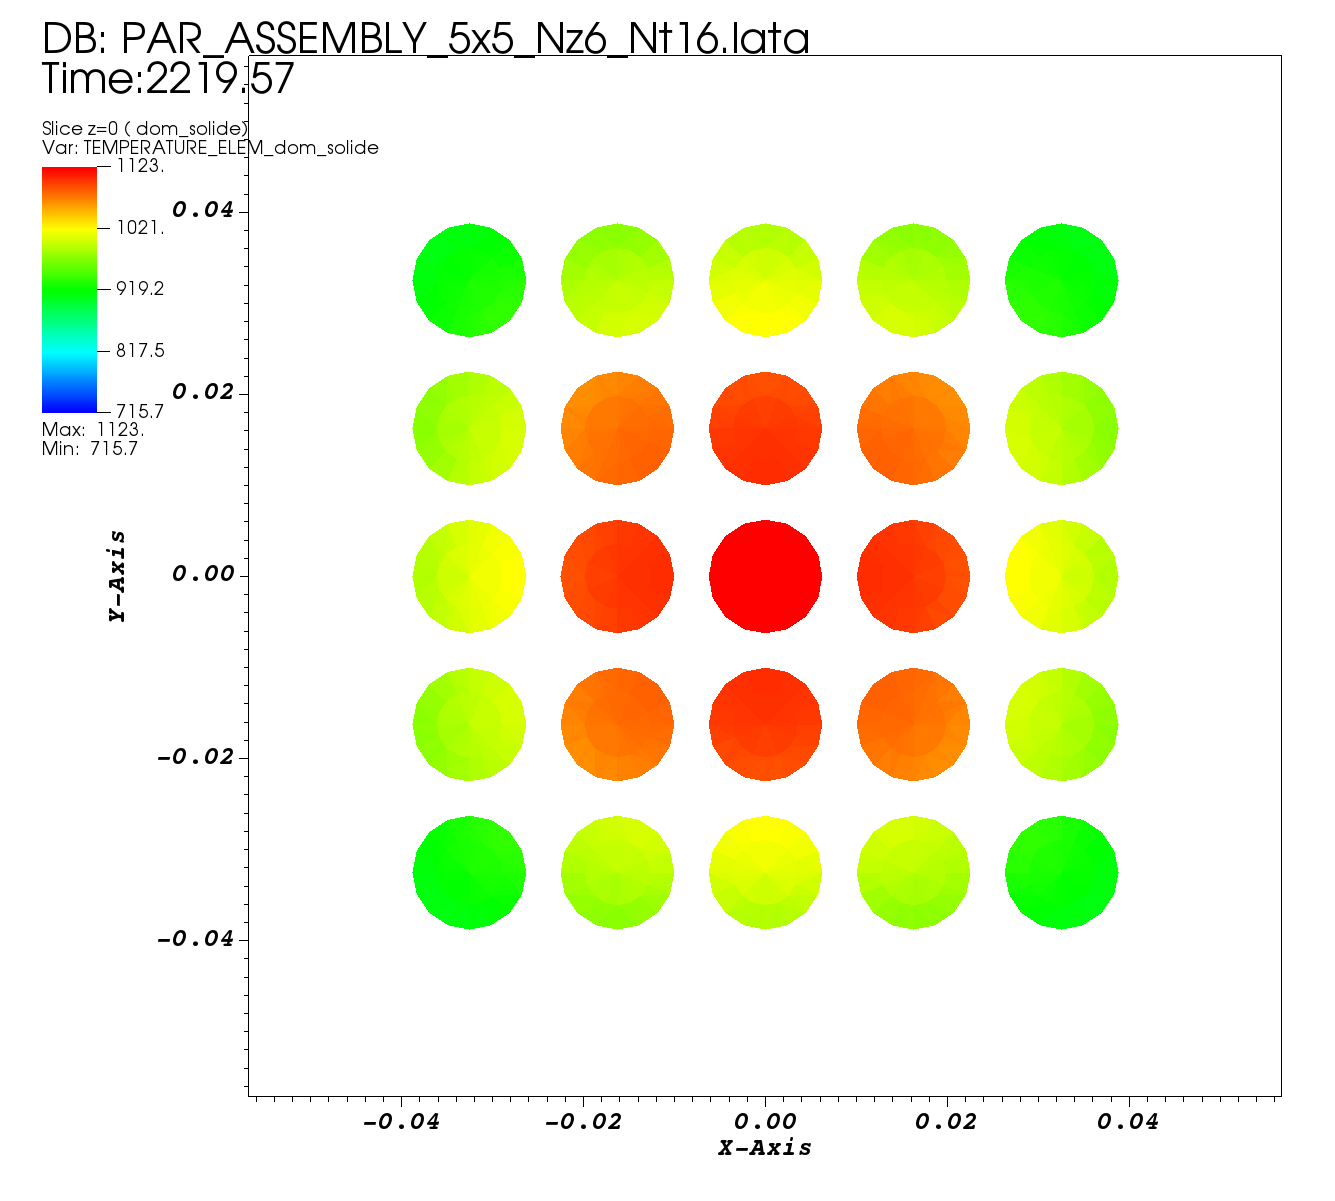
\includegraphics[width=\linewidth]{PICTURES/c5couplage/slicez0.png}
\end{minipage}
\hfill
\begin{minipage}{0.45\textwidth}
    \centering
    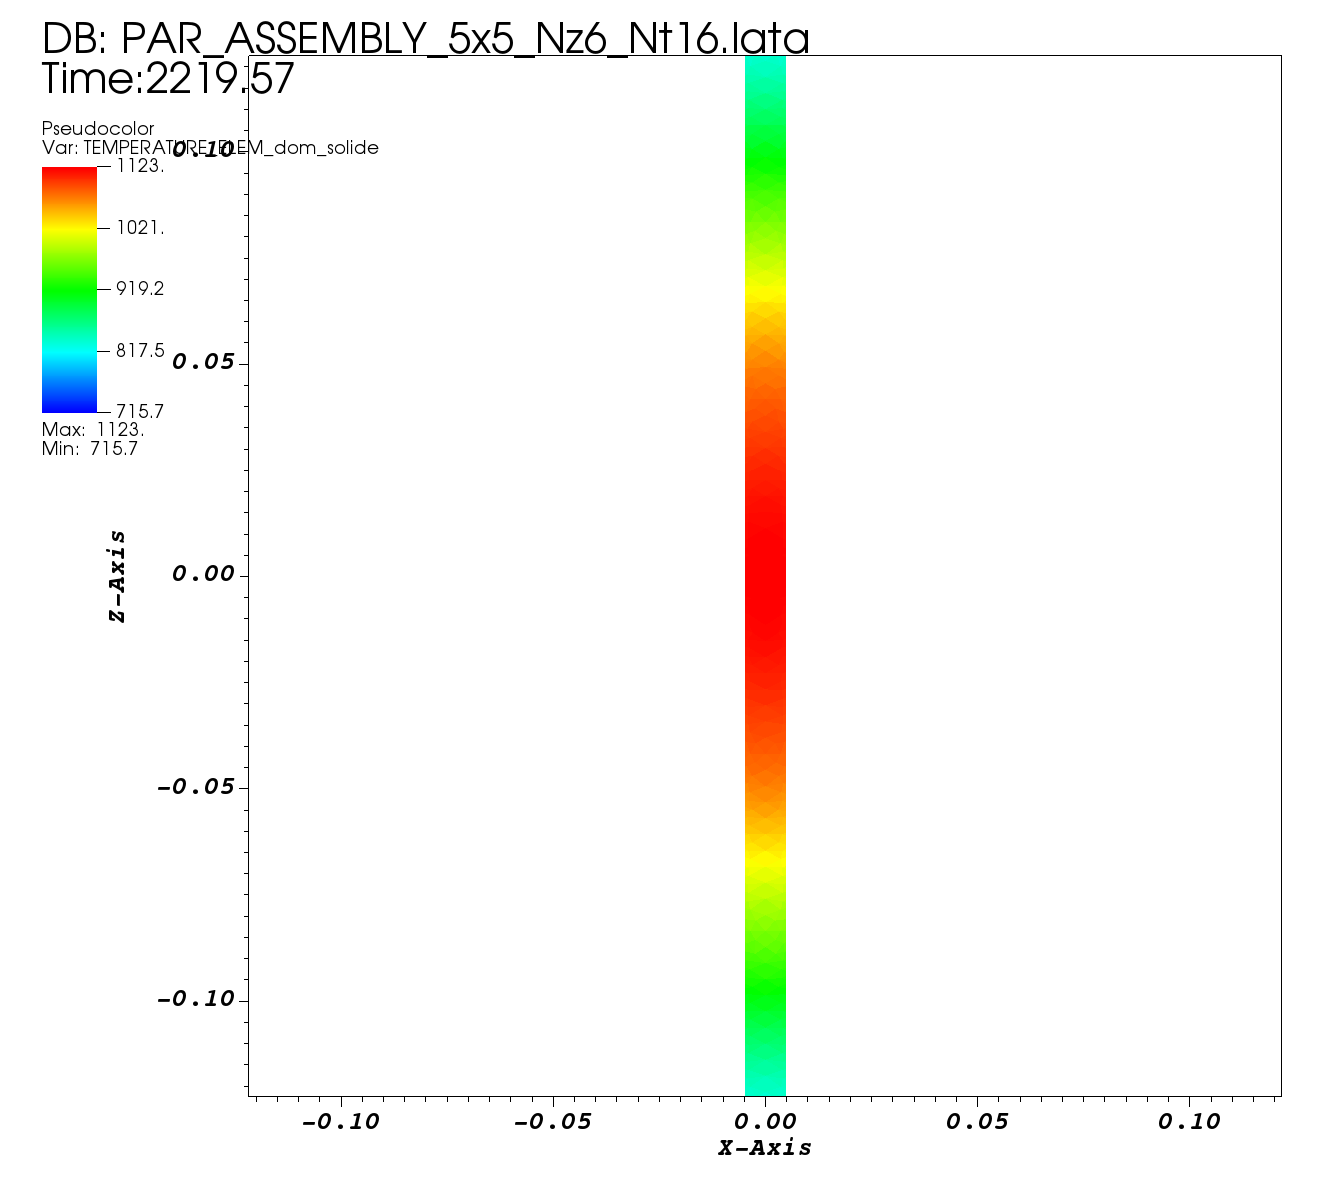
\includegraphics[width=\linewidth]{PICTURES/c5couplage/sliceMid.png}
\end{minipage}
\caption{Plan de coupe en $Z=0$ (gauche) et coupe verticale du crayon central (droite).}
\label{fig:domaine}
\end{figure}

Le combustible et le fluide caloporteur sont caractérisés par les propriétés thermophysiques et radiatives résumées dans le Tableau~\ref{tab:proprietes}. Trois niveaux de puissance volumique sont déposés dans le combustible, modulés selon un profil axial en cosinus caractéristique de la distribution de puissance neutronique le long d'un crayon combustible ; aucune source de puissance n'est imposée dans le fluide. Ces trois cas, résumés dans le Tableau~\ref{tab:puissances}, correspondent à des températures moyennes croissantes du crayon central, permettant d'étudier l'effet de la discrétisation sur une gamme de régimes thermiques représentative. Le fluide est par ailleurs traité sous l'hypothèse de Boussinesq, avec une gravité orientée selon $-\vec{z}$. Une température de paroi $T_{\mathrm{paroi}} = 600$~K est imposée en périphérie du domaine.

\begin{table}[H]
\centering
\begin{tabular}{ccc}
\toprule
Cas & Puissance volumique~[$\mathrm{MW/m^3}$] & $T_{\mathrm{moy}}$ crayon central~[K] \\
\midrule
1 & $3$  & $1013$ \\
2 & $4$  & $1080$ \\
3 & $45$ & $2089$ \\
\bottomrule
\end{tabular}
\caption{Niveaux de puissance volumique étudiés et température moyenne résultante du crayon central.}
\label{tab:puissances}
\end{table}

\begin{table}[H]
\centering
\begin{tabular}{lccc}
\toprule
Propriété & Symbole & Combustible & Fluide \\
\midrule
Masse volumique & $\rho$~[$\mathrm{kg/m^3}$] & $10\,110$ & $6{,}754\times10^{-5}$ \\
Conductivité thermique & $\lambda$~[$\mathrm{W/(m.K)}$] & $10$ & $0{,}01$ \\
Capacité calorifique & $C_p$~[$\mathrm{J/(kg.K)}$] & $350$ & $1141{,}1$ \\
Viscosité dynamique & $\mu$~[$\mathrm{Pa.s}$] & -- & $4{,}153\times10^{-5}$ \\
Coefficient de dilatation thermique & $\beta_{\mathrm{th}}$~[$\mathrm{K^{-1}}$] & -- & $10^{-3}$ \\
Émissivité & $\epsilon$ & $1$ & -- \\
\bottomrule
\end{tabular}
\caption{Propriétés thermophysiques et radiatives du combustible et du fluide caloporteur.}
\label{tab:proprietes}
\end{table}

\subsection{Maillage}

Le maillage surfacique des crayons est généré à l'aide de l'algorithme \texttt{MG-CADSurf} de la plateforme \textsc{Salome}, avec une taille de maille cible comprise entre $2$~mm et $10$~mm. Ce maillage de surface constitue le support du calcul des facteurs de vue par lancer de rayons. Le maillage volumique du domaine fluide, nécessaire à la résolution du problème thermohydraulique dans TRUST, est ensuite généré à partir de ce maillage surfacique à l'aide de l'algorithme tétraédrique \texttt{MG-Tetra}, et comporte environ $1{,}2$ million d'éléments. La Figure~\ref{fig:mesh} présente une coupe horizontale et une coupe verticale de ce maillage.

\begin{figure}[H]
\centering
\begin{minipage}{0.45\textwidth}
    \centering
    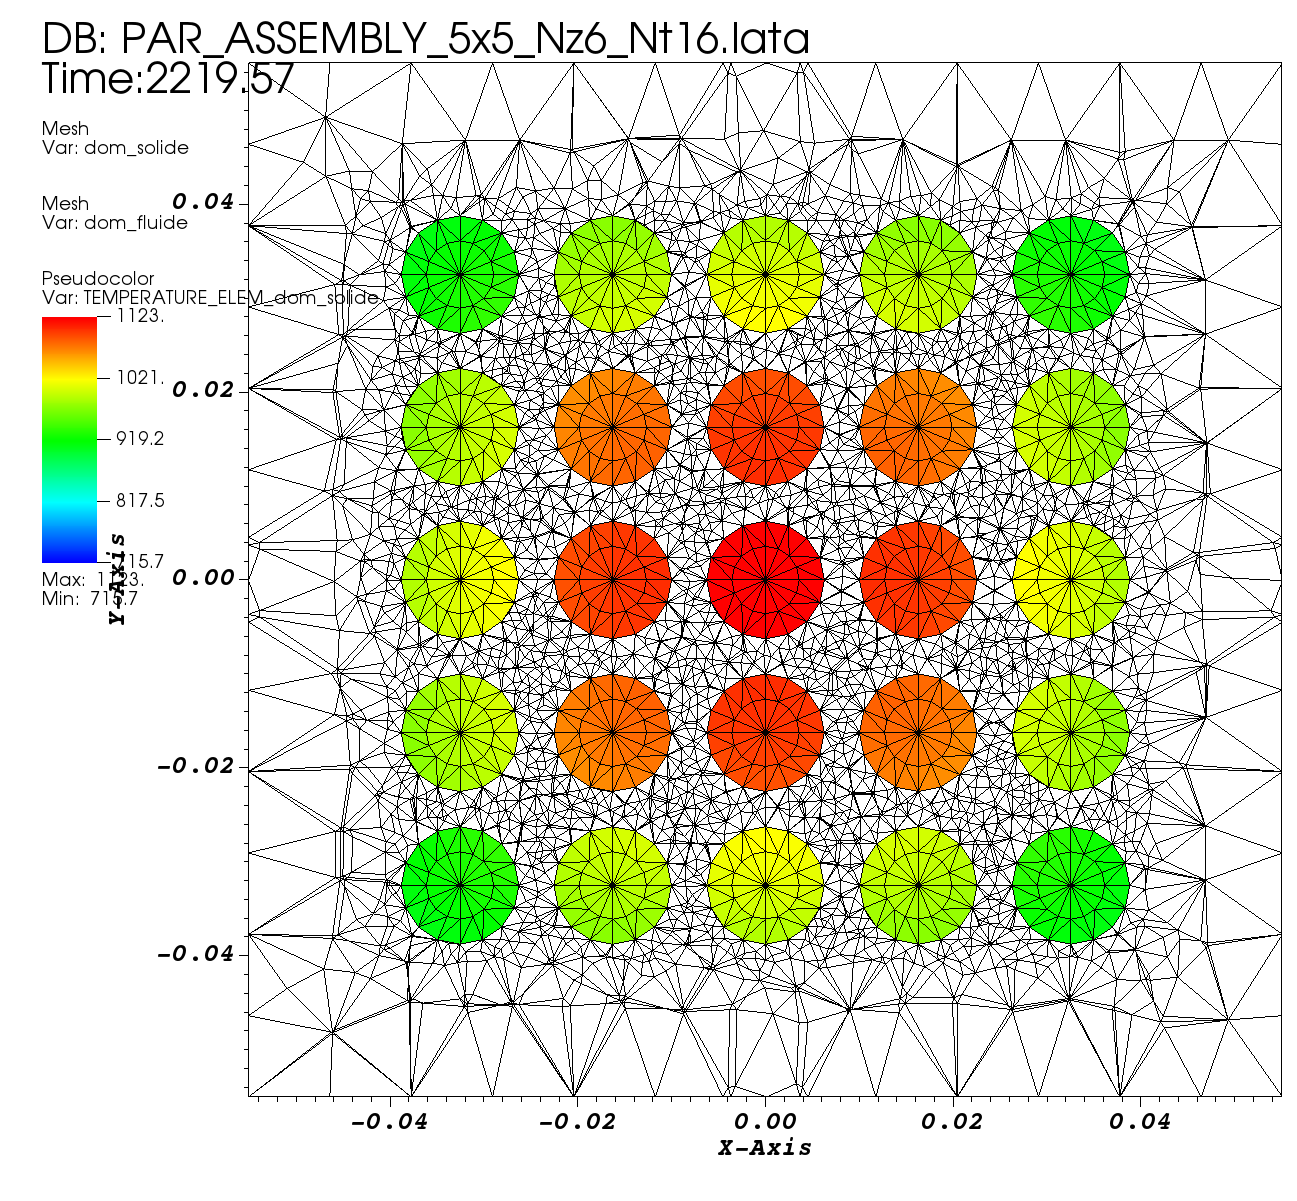
\includegraphics[width=\linewidth]{PICTURES/c5couplage/mesh_horizontal.png}
\end{minipage}
\hfill
\begin{minipage}{0.45\textwidth}
    \centering
    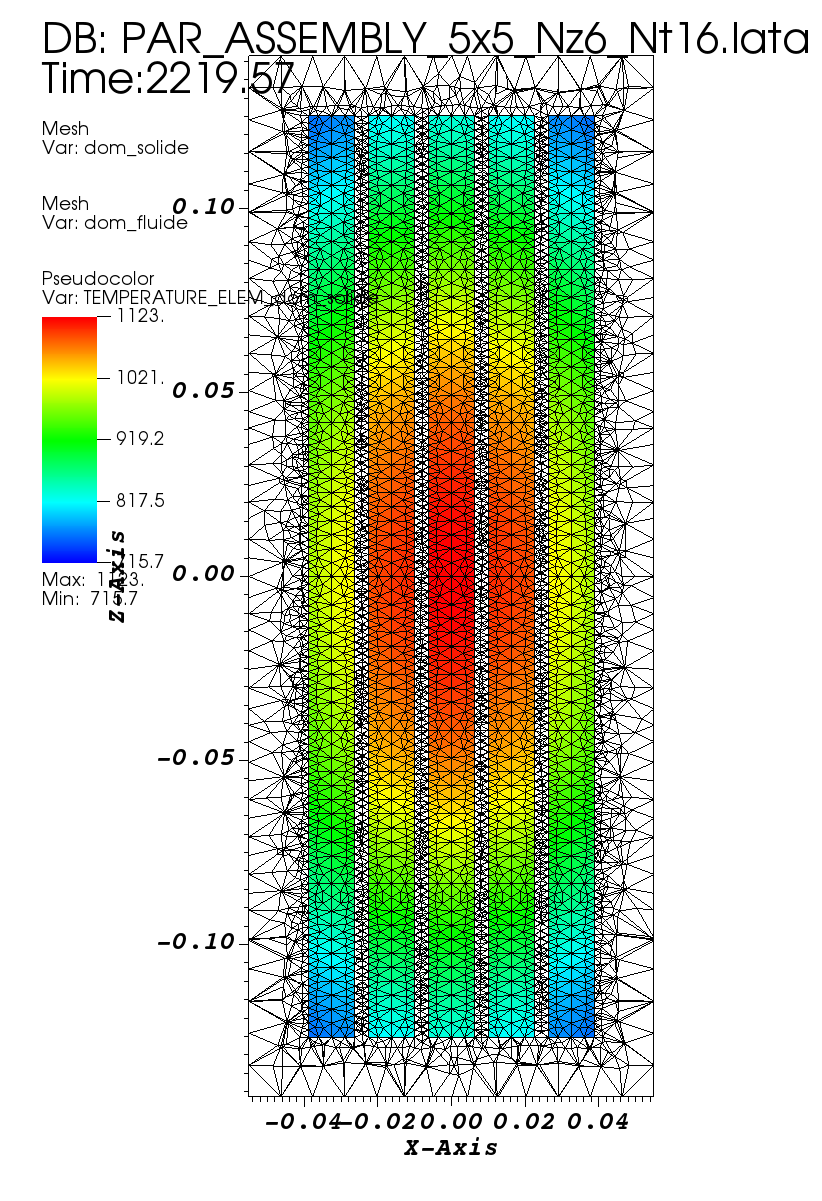
\includegraphics[width=\linewidth]{PICTURES/c5couplage/mesh_vertical.png}
\end{minipage}
\caption{Coupe horizontale en $Z=0$ (gauche) et coupe verticale (droite) du maillage volumique.}
\label{fig:mesh}
\end{figure}

Afin d'étudier l'effet de la discrétisation géométrique sur les résultats, la surface de chaque crayon est en outre discrétisée, pour les besoins du calcul radiatif, selon $N_\theta$ secteurs angulaires et $N_z$ tranches axiales, formant ainsi $N_\theta \times N_z$ sous-surfaces élémentaires par crayon. Le nombre de secteurs angulaires est fixé à $N_\theta = 16$ pour l'ensemble de cette étude. Le nombre de tranches axiales $N_z$, seul paramètre variable, est balayé sur la plage résumée dans le Tableau~\ref{tab:nz_values}, afin de quantifier le biais introduit par l'hypothèse de radiosité uniforme.

\begin{table}[H]
\centering
\begin{tabular}{lc}
\toprule
Paramètre & Valeurs testées \\
\midrule
$N_z$ & $2, 4, 6, \dots, 20$ \\
\bottomrule
\end{tabular}
\caption{Valeurs du nombre de tranches axiales $N_z$ étudiées.}
\label{tab:nz_values}
\end{table}


\subsection{Stratégie de résolution numérique}

Le problème thermohydraulique couplé est résolu dans \trust par une méthode de volumes finis. Bien que l'objectif de cette étude soit d'obtenir l'état stationnaire du système, \trust résout ce problème par une approche de marche en temps : le schéma numérique fait converger la solution vers un point fixe stationnaire par intégration temporelle successive, plutôt que par une résolution directe du problème stationnaire.

Le schéma retenu est un schéma d'Euler implicite, dont le pas de temps $dt$ est piloté automatiquement entre les bornes $dt_{\mathrm{min}}$ et $dt_{\mathrm{max}}$ par un facteur de sécurité \texttt{facsec}. Ce facteur ajuste le pas de temps à chaque itération en fonction de la vitesse de convergence du solveur implicite, permettant d'accélérer la marche en temps tant que la convergence du système linéaire reste satisfaisante. Les principaux paramètres du schéma sont résumés dans le Tableau~\ref{tab:solveur}.

\begin{table}[H]
\centering
\begin{tabular}{lcc}
\toprule
Paramètre & Symbole/mot-clé & Valeur \\
\midrule
Pas de temps minimal & $dt_{\mathrm{min}}$ & $10^{-3}$~s \\
Pas de temps maximal & $dt_{\mathrm{max}}$ & $10^{3}$~s \\
Facteur de sécurité & \texttt{facsec} & $10^{7}$ -- $10^{8}$ \\
Facteur de sécurité maximal & \texttt{facsec\_max} & $10^{8}$ -- $10^{9}$ \\
Seuil de convergence (solveur linéaire) & -- & $10^{-1}$ \\
Seuil de convergence (schéma implicite) & -- & $10^{-1}$ \\
Seuil de stationnarité & \texttt{seuil\_statio} & $10^{-5}$ \\
\bottomrule
\end{tabular}
\caption{Paramètres du schéma temporel implicite utilisé pour la convergence vers l'état stationnaire.}
\label{tab:solveur}
\end{table}

La valeur de \texttt{facsec} retenue, très supérieure à l'unité, illustre bien la nature de cette stratégie : le pas de temps n'est plus piloté par un critère de précision physique de la dynamique transitoire, mais uniquement par la vitesse à laquelle le solveur implicite parvient à converger à chaque itération. Cette approche revient ainsi à utiliser l'intégration temporelle comme un simple outil numérique permettant d'atteindre efficacement l'état stationnaire recherché, sans chercher à représenter fidèlement une éventuelle dynamique transitoire réelle du système. Le calcul est considéré comme convergé lorsque l'évolution de la solution entre deux pas de temps successifs devient inférieure au seuil de stationnarité \texttt{seuil\_statio}.